\documentclass[a4paper]{article}
\usepackage{fullpage, graphicx, array}

\begin{document}
\title{G52SOF - Software Requirements Specification}
\author{Harry Coupe, PSYHC5, 4321806}
\maketitle
\pagebreak

\tableofcontents

\addcontentsline{toc}{section}{Revision History}
\section* {Revision History}
\begin{tabular}{|m{1.5cm}|m{1.5cm}|m{9cm}|m{1.5cm}|}
	\hline
	\textbf{Name} & \textbf{Date} & \textbf{Reason For Change} & \textbf{Version}\\
	\hline
	 Harry & 14/05/20 & Initial version of SRS completed & v0.1 \\ 
	\hline
	 & & & \\
	\hline
	 & & & \\
	\hline 
\end{tabular}	
\pagebreak


\section {Introduction}
\subsection {Purpose}
The product that has been commissioned by a universities well-being team is an android application to aid students in dealing with assessment and exam time stress. In the current version v0.1 the requirements of the 3 main sections of the app will be discussed: calender, advice section, exercise section.


\subsection {Product Scope}
As seen in the vision and scope document the app is being made to help students dealing with stress during assessment periods using a calender for deadline/date management, a section containing exercises to aid in dealing with stress and a section where advice is readily available.

\subsection{Intended Audience and Reading Suggestions}
This project is commissioned by the university well-being team so this document is for the development team and the review of their team.

\section {Overall Description}
\subsection {Product Perspective}
This new self-contained product is being commissioned by a universities well-being team as a way for them to be able to aid their students in dealing with the extremely stressful periods they are put under in the current education system. 

\subsection {Product Functions}
The main functions of this app would be:
\begin{itemize}
	\item A calender that will allow students to add and edit deadlines.
	\item A section where advice is available to students dealing with these issues.
	\item A section where exercises are available to aid in dealing with stress.
\end{itemize}
The finer details of these features will be discussed further below.
\pagebreak

\subsection{User Class and Characteristics}
The system will support 3 types of users: Student, Teacher and Trusted User. The student will be able to:
\begin{itemize}
	\item Will be able to organise and edit their deadlines within valid dates and be able to have the app alert them close to the time of these deadlines. 
	\item Will have access to information about exercises that aid with the relief of stress. 
	\item Will be able to access advice through either: live chat with well-being teams, Helplines and a message board system where users can share experiences and advice
\end{itemize}
The Teacher will be able to:
\begin{itemize}
	\item Add deadlines for a group of students to receive on their calendar
	\item Edit deadlines their students have received from them
	\item Alert students about upcoming deadlines
\end{itemize}
The Trusted User will be able to:
\begin{itemize}
	\item Add exercise guides for students to follow
	\item Add advice for students on the app
	\item Edit their posts on the platform
\end{itemize}
 
\pagebreak

\section {External Interface Requirements}
\subsection {User Interfaces}
\begin{itemize}
	\item Front-end Software: React
	\item Back-end Software: Node.js
\end{itemize}
The main form of user interface within the app will be through a Navigation Bar on the left hand side opened by a menu button in the bottom right. Through this bar there will be options to all 3 different sections and a settings section. The other interface will be through buttons to details on sections or adding/editing deadlines in the calender section. Said navigation bar is detailed bellow from a screenshot of the prototypes version of it.
\begin{figure}[h!]
	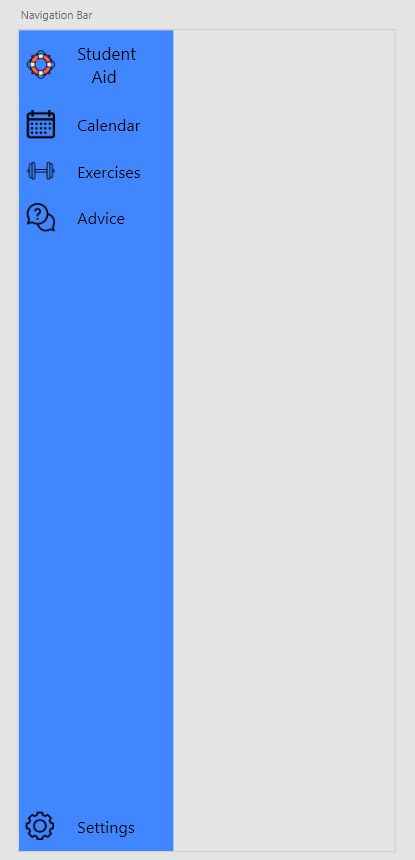
\includegraphics[scale=0.5]{NavBar.png}
	\caption{A screenshot of the navigation bar in the prototype}
	\label{fig:Prototype Navigation Bar}
\end{figure}

\subsection{Hardware Interfaces}
\begin{itemize}
	\item Android OS
\end{itemize}
\pagebreak


\section {System Features}	
Requirement labelling: (feature - id number - priority)\\
Priority is labelled with 1-9, 1 being low and 9 being high.
\subsection{Organisational Calendar}
\subsubsection*{Functional Requirements}
	(CAL-001-9) The application shall not allow users to add deadline events to an invalid date.\\
	(CAL-002-9) The application shall allow users to create new deadline events on valid dates.\\
	(CAL-003-9) The application shall allow users to edit existing deadline events on valid dates.\\
	(CAL-004-5) The application shall allow mobile alerts to be set relating to deadline events.\\
	(CAL-005-7) The application shall allow deadline events to be set to exams or assessments.\\
	(CAL-006-4) The application shall allow teacher users to create groups of students to send deadlines to.\\
	(CAL-007-4) The application shall allow the user, if the user is in a valid group, to receive deadlines from teachers. \\
	(CAL-008-3) The application shall allow the user the export or sync the calendar data to external calendar apps.\\
	
\subsection{Recommended Exercise}
\subsubsection*{Functional Requirements}
	(EXC-001-9) The application shall give users access to trusted information on exercises to help them\\
	(EXC-002-5) The application shall allow users to give a thumbs up rating on exercises they find useful\\
	(EXC-003-5) The application shall allow users to give a thumbs down rating on exercises they did not find useful\\
	(EXC-004-9) The application shall allow trusted users to add exercise information for users\\
	(EXC-005-8) The application shall allow trusted users to edit their additions to the platform\\
	(EXC-006-x) \\
	(EXC-007-x) \\
	(EXC-008-x) \\
	
\subsection{Help and Advice}
\subsubsection*{Functional Requirements}
	(ADV-001-7) The application shall allow users to talk to well-being team members when available via live chat\\
	(ADV-002-9) The application shall give users contact information for relevant organisations to help with their issues\\
	(ADV-003-8) The application shall allow users to add topics to the message board\\
	(ADV-004-8) The application shall allow users to edit their topics on the message board\\
	(ADV-005-8) The application shall allow users to reply to other users topics\\
	(ADV-006-6) The application shall allow users to vote on how useful a topic is\\
	(ADV-007-x) \\
	(ADV-008-x) \\	

\section {Other Nonfunctional Requirements}
\subsection {Performance Requirements}
The application will be responsive and any refresh or load will be beneath 1000ms where possible and bellow 3000ms in almost all situations. This is in place as users have fairly low patience when it comes to load times so to retain users we gain a key factor to this is keeping load times low. \\

\noindent The application will be light weight when running, using bellow 500mb of the devices memory at all times to aid the responsiveness of the application but also to avoid any crashes due to the over allocation of memory on mobile devices.
\pagebreak






\end{document}